% !TeX spellcheck = en_GB
% !TeX program = lualatex
%
% v 2.3  Feb 2019   Volker RW Schaa
%		# changes in the collaboration therefore updated file "jacow-collaboration.tex"
%		# all References with DOIs have their period/full stop before the DOI (after pp. or year)
%		# in the author/affiliation block all ZIP codes in square brackets removed as it was not %         understood as optional parameter and ZIP codes had bin put in brackets
%       # References to the current IPAC are changed to "IPAC'19, Melbourne, Australia"
%       # font for ‘url’ style changed to ‘newtxtt’ as it is easier to distinguish "O" and "0"
%
\documentclass[%              % paper size definition not needed as JACoW page size is set
               %boxit,        % show page boundaries to check whether paper is inside correct margins
               %refpage       % references placed on separate page
               %biblatex,     % BibLaTeX is to be used
               %nospread,     % flushend option: do not fill with whitespace to balance columns
               %hyphens,      % allow \url to hyphenate at "-" (hyphens)
               %luatex,       % use LuaLaTeX to process the file
               ]{jacow}
%
% Allow compilation from repo root or TEXPaper folder
\graphicspath{{2026/IPAC'26 France/TEXPaper/}{2026/IPAC'26 France/TEXPaper/img/}{img/}}
%
% CHANGE SEQUENCE OF GRAPHICS EXTENSION TO BE EMBEDDED
% ----------------------------------------------------
% test for XeTeX where the sequence is by default eps-> pdf, jpg, png, pdf, ...
%    and the JACoW template provides JACpic2v3.eps and JACpic2v3.jpg which
%    might generates errors, therefore PNG and JPG first
%
\makeatletter%
	\ifboolexpr{bool{xetex}}
	 {\renewcommand{\Gin@extensions}{.pdf,%
	                    .png,.jpg,.bmp,.pict,.tif,.psd,.mac,.sga,.tga,.gif,%
	                    .eps,.ps,%
	                    }}{}
\makeatother

% CHECK FOR XeTeX/LuaTeX BEFORE DEFINING AN INPUT ENCODING
% --------------------------------------------------------
%   utf8  is default for XeTeX/LuaTeX
%   utf8  in LaTeX only realises a small portion of codes
%
\ifboolexpr{bool{xetex} or bool{luatex}} % test for XeTeX/LuaTeX
 {}                                      % input encoding is utf8 by default
 {\usepackage[utf8]{inputenc}}           % switch to utf8

\usepackage[english]{babel}

%
% if BibLaTeX is used
%
\ifboolexpr{bool{jacowbiblatex}}%
 {%
  \addbibresource{jacow-test.bib}
  \addbibresource{biblatex-examples.bib}
 }{}
\listfiles

%%
%%   Lengths for the spaces in the title
%%   \setlength\titleblockstartskip{..}  %before title, default 3pt
%%   \setlength\titleblockmiddleskip{..} %between title + author, default 1em
%%   \setlength\titleblockendskip{..}    %afterauthor, default 1em

\begin{document}

\title{Spin Coherence Time Optimization by Mapping Method}

\author{S. Kolokolchikov\textsuperscript{1,2}, A. Aksentyev\textsuperscript{1,2,3}, A. Melnikov\textsuperscript{1,2,4}, P. Palamarchuka\textsuperscript{1,3}, Y. Senichev\textsuperscript{1,2} \\
\textsuperscript{1}Institute for Nuclear Research of the Russian Academy of Sciences, Moscow, Russia\\
\textsuperscript{2}Moscow Center for Advanced Studies, Moscow, Russia\\
\textsuperscript{3}National Research Nuclear University MEPhI, Moscow, Russia\\
\textsuperscript{4}Landau Institute for Theoretical Physics, Chernogolovka, Russia\\}
	
\maketitle

%
\begin{abstract}
A sufficiently long Spin Coherence Time (SCT) is a fundamental requirement for precision measurements of the electric dipole moment (EDM) of charged particles in storage rings. SCT optimization is performed using three sextupole families that suppress second-order effects arising from emittance and momentum spread. These sextupoles are placed at the maxima of the beta functions in both planes and in regions with significant horizontal dispersion. The study examines the capability of the mapping method to simultaneously suppress spin decoherence and achieve zero chromaticity in both transverse planes in magnetic, electrostatic, and combined-function structures.
\end{abstract}

\section{Introduction}
\par A sufficiently long spin coherence time (SCT) is a prerequisite for storage-ring electric dipole moment (EDM) experiments~\cite{melnikov22,senichev25}. Operationally, SCT is tied to the spread of equilibrium orbit length (path lengthening) over betatron amplitudes and momentum offset within the bunch; the practical route to coherence is to correct that lengthening, which simultaneously tames the chromatic and higher-order spin--orbit effects driven by the same optics. Prototype rings continue to explore concrete optimisation strategies~\cite{shankar23}.
\par Mitigating that lengthening in second order is precisely what motivates three sextupole families, located near extrema of the horizontal and vertical beta functions and in regions with significant horizontal dispersion. Three such families are \emph{necessary} so that \(\xi_x\), \(\xi_y\), and the longitudinal chromatic integral \(\eta_1\) can be adjusted independently; for each of the three magneto-optical structures below, the layout is chosen so that the linearised response from the family currents to \((\xi_x,\xi_y,\eta_1)\) remains invertible in the scanned range. Zeroing transverse chromaticity in a magnetic storage ring was shown experimentally to greatly lengthen in-plane polarisation lifetime~\cite{guidoboni18}.
\par The studies reported here were performed with COSY Infinity~\cite{cosy}; supporting scripts, notebooks, and lattice files are collected in Ref.~\cite{sctrepo}. The paper summarises the linear mapping construction, documents the three lattices, and analyses how \(\Delta\nu_s\) depends on \(\xi_x\), \(\xi_y\), and \(\eta_1\).

\section{Mapping method}
\subsection{Scan and observables}
\par Nested COSYScript loops scan the strengths of the three sextupole families. At each grid point the analysis uses two modes: chromaticities \(\xi_x\) and \(\xi_y\) are evaluated in order \texttt{OV 3 2 1} (tune shifts after the transformation to the momentum-dependent fixed point), while the longitudinal chromatic integral \(\eta_1\) and spin-transfer data for the probes use order \texttt{OV 3 3 0}. For each probe, small initial amplitudes in \(x\), \(y\), and \(\Delta K/K\) are specified and evaluated at two levels per direction so that the induced response can be read off; the one-turn linear spin map of the ring is applied to the initial spin degrees of freedom rather than stepping the orbit symplectically. Components \(\Delta\vec\nu_s=(\Delta\nu_x,\Delta\nu_y,\Delta\nu_z)^T\) are then recorded relative to the reference particle on the closed orbit. After the scan, ordinary least squares fits linear models in the excitation vector \(\vec I\) to \(\vec\xi\) and to each \(\Delta\nu_k\) so that the Jacobian-based mapping of Sec.~\ref{subsec:linresp} can be built.
\par Each sampled machine state is labelled by \(\vec I=(I_{x1},I_{x2},I_{y1})^T\). We record:
\begin{itemize}
	\item chromatic observables \(\vec\xi = (\xi_x,\xi_y,\eta_1)^T\);
	\item components \(\Delta\vec\nu_s=(\Delta\nu_x,\Delta\nu_y,\Delta\nu_z)^T\) for the phase-space probes defined above.
\end{itemize}

\subsection{Linear response model}
\label{subsec:linresp}
\par Around the scanned range, we approximate both the chromatic observables and the spin response by a linear model:
\begin{equation}
	\vec\xi = \mathbf{R}_{int}\,\vec I + \vec\xi_{nat},\qquad
	\Delta\vec\nu_s = \mathbf{R}_{spin}\,\vec I + \Delta\vec\nu_{s,nat},
	\label{eq:lin_model}
\end{equation}
\noindent where \(\vec\xi_{nat}\) and \(\Delta\vec\nu_{s,nat}\) are the intercepts of the linear model relative to the scan baseline. The matrices \(\mathbf{R}_{int}\) and \(\mathbf{R}_{spin}\) are the slope blocks obtained by ordinary least squares with a design matrix consisting of the three family strengths and a constant column.

\subsection{Control law and transfer operator}
\par For a target chromatic state \(\vec\xi_{t}\), the required sextupole setting is computed as
\begin{equation}
	\vec I = \mathbf{R}_{int}^{-1}\left(\vec\xi_{t}-\vec\xi_{nat}\right),
	\label{eq:control_law}
\end{equation}
\noindent and substituted into Eq.~(\ref{eq:lin_model}) to obtain a direct map from chromaticity to spin response:
\begin{equation}
	\Delta\vec\nu_s
	= \underbrace{\left(\mathbf{R}_{spin}\mathbf{R}_{int}^{-1}\right)}_{\mathbf{S}}
	\left(\vec\xi_{t}-\vec\xi_{nat}\right)+\Delta\vec\nu_{s,nat}.
	\label{eq:transfer}
\end{equation}
\noindent The composite matrix \(\mathbf{S}\) is the Jacobian linking chromatic targets to the spin-tune response used when comparing lattices.

\subsection{Decoupled plane-by-plane scans}
\par To isolate the dominant mechanisms, we perform scans in \(\xi_x\), \(\xi_y\), and \(\eta_1\) while constraining the other two components to zero:
\begin{align}
	&(\xi_x, \xi_y, \eta_1) = (\xi_x,0,0), \nonumber\\
	&(\xi_x, \xi_y, \eta_1) = (0,\xi_y,0), \nonumber\\
	&(\xi_x, \xi_y, \eta_1) = (0,0,\eta_1).
	\label{eq:constraints}
\end{align}
\noindent In practice, this means solving Eq.~(\ref{eq:control_law}) for each scan point, with \(\vec\xi_t\) constructed according to Eq.~(\ref{eq:constraints}). The transfer curves are evaluated on dense target grids within the scanned intervals used in COSY Infinity, here \(\xi_x,\xi_y\in[-10,10]\) and \(\eta_1\in[-1,1]\).

\section{Lattice benchmarks and \(\Delta\nu_s\) versus chromaticity}
\par Figures~\ref{fig:m2p_xz}--\ref{fig:n8_xz} show \(\Delta\nu_s\) versus chromatic targets from Eqs.~(\ref{eq:control_law})--(\ref{eq:transfer}) with the decoupled constraints of Eq.~(\ref{eq:constraints}), for the nominal and larger excursions defined above. The three layouts below---magnet-only, electrostatic, and combined-function QFS---use the same sextupole scan and fitting protocol.

\subsection{Magnet-only ring}
\par The magnet-only benchmark is a compact purely magnetic ring used as the conventional baseline; Twiss functions are in Fig.~\ref{fig:twiss_m2p}.
\begin{figure}[!tbh]
	\centering
	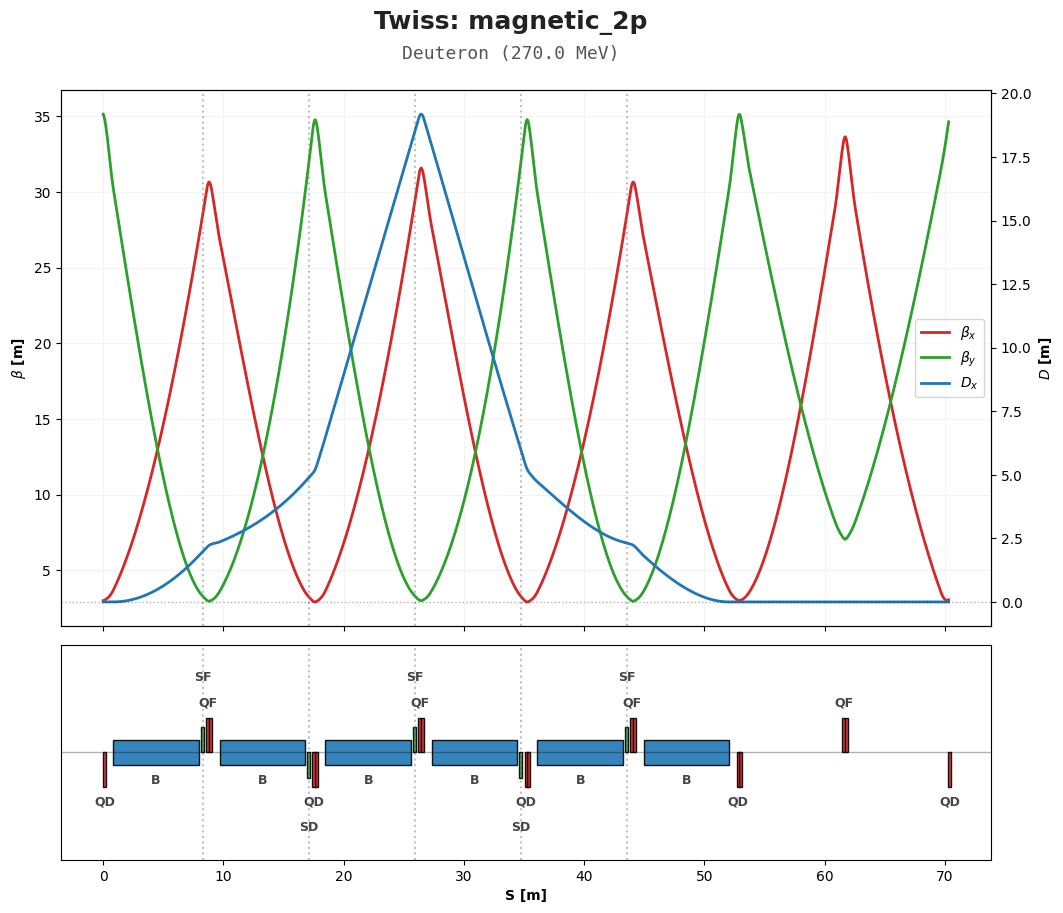
\includegraphics[width=\columnwidth]{img/TUP3065_f7}
	\caption{Magnet-only ring: Twiss functions.}
	\label{fig:twiss_m2p}
\end{figure}
\begin{figure}[!tbh]
	\centering
	\begin{minipage}[t]{0.49\columnwidth}
		\centering
		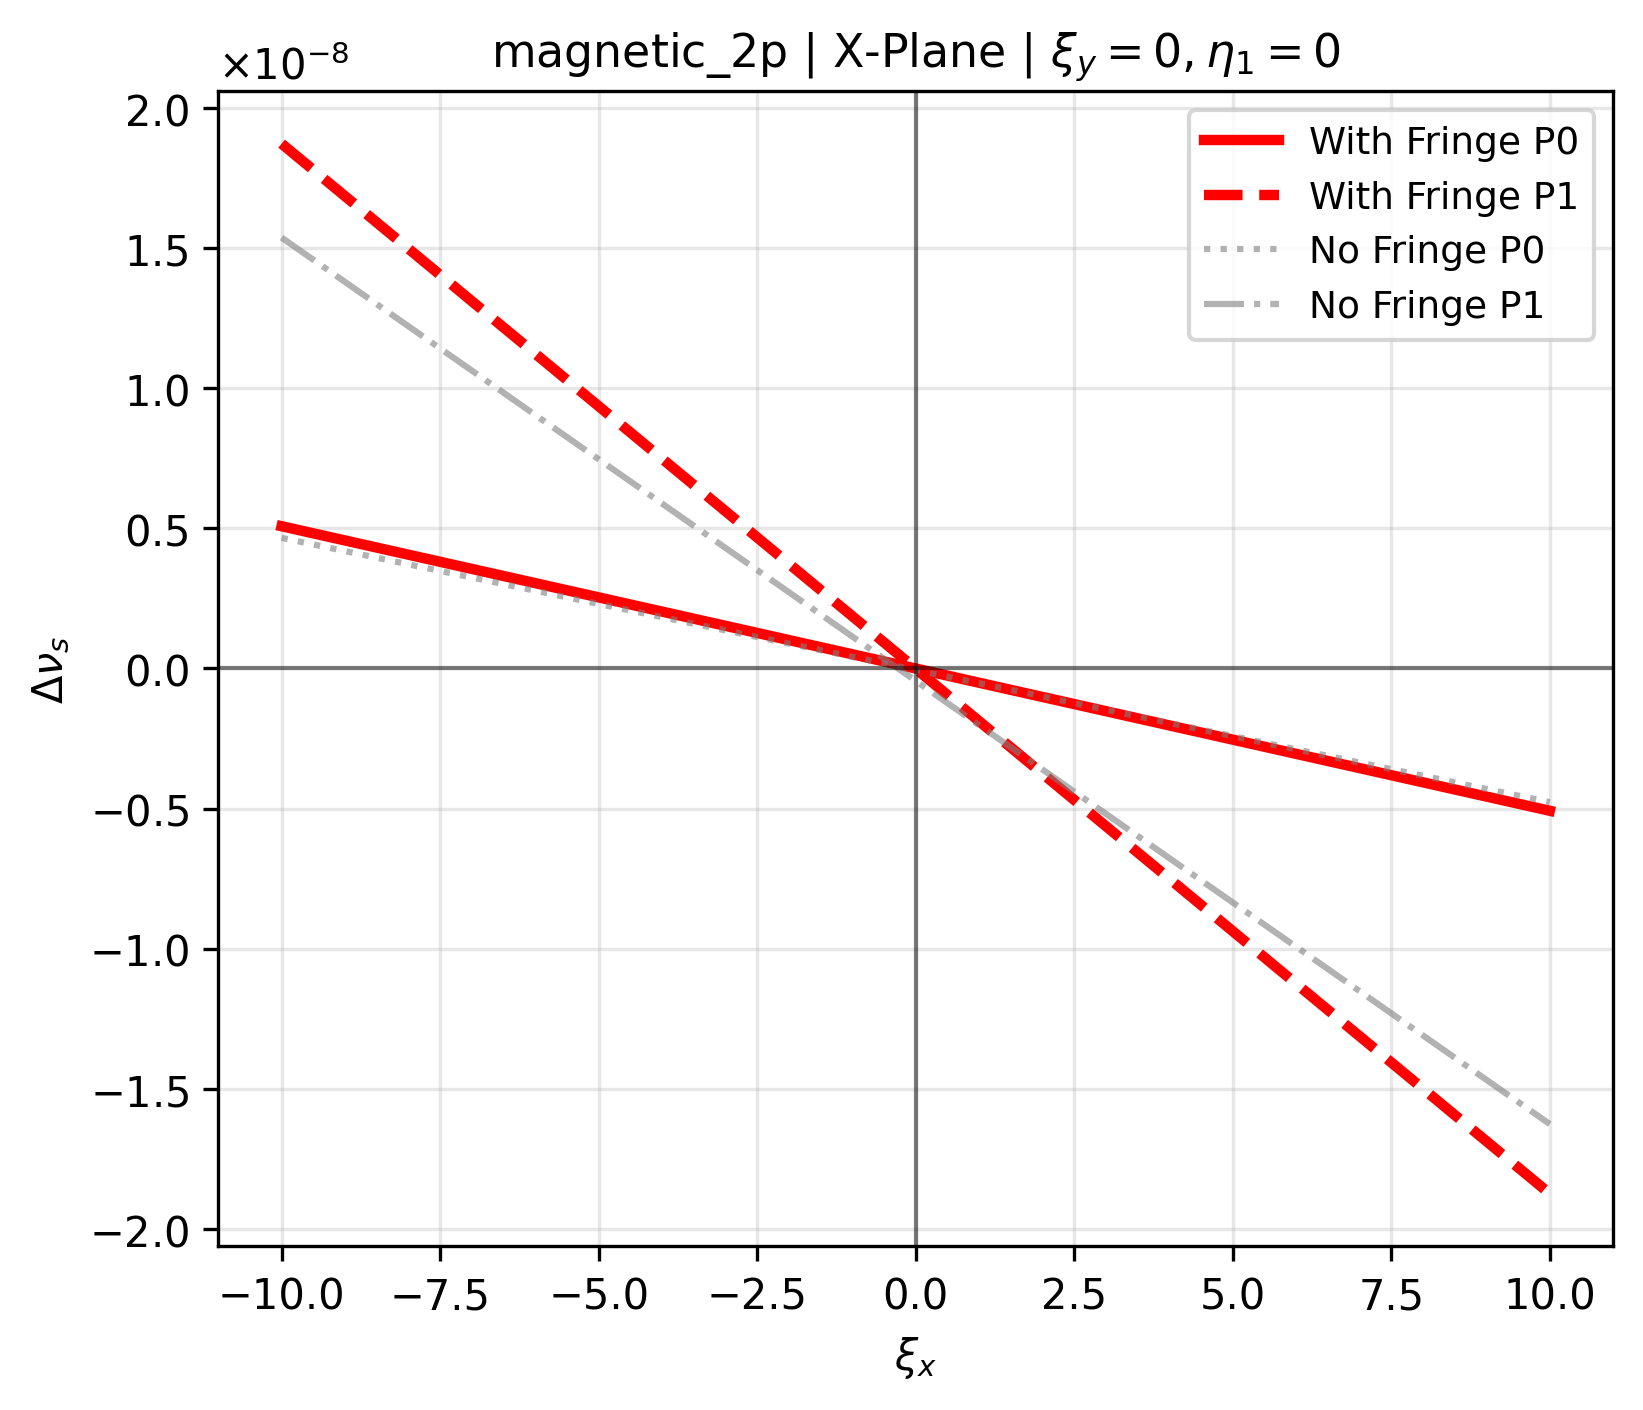
\includegraphics[width=\linewidth]{img/TUP3065_f1}
	\end{minipage}\hfill
	\begin{minipage}[t]{0.49\columnwidth}
		\centering
		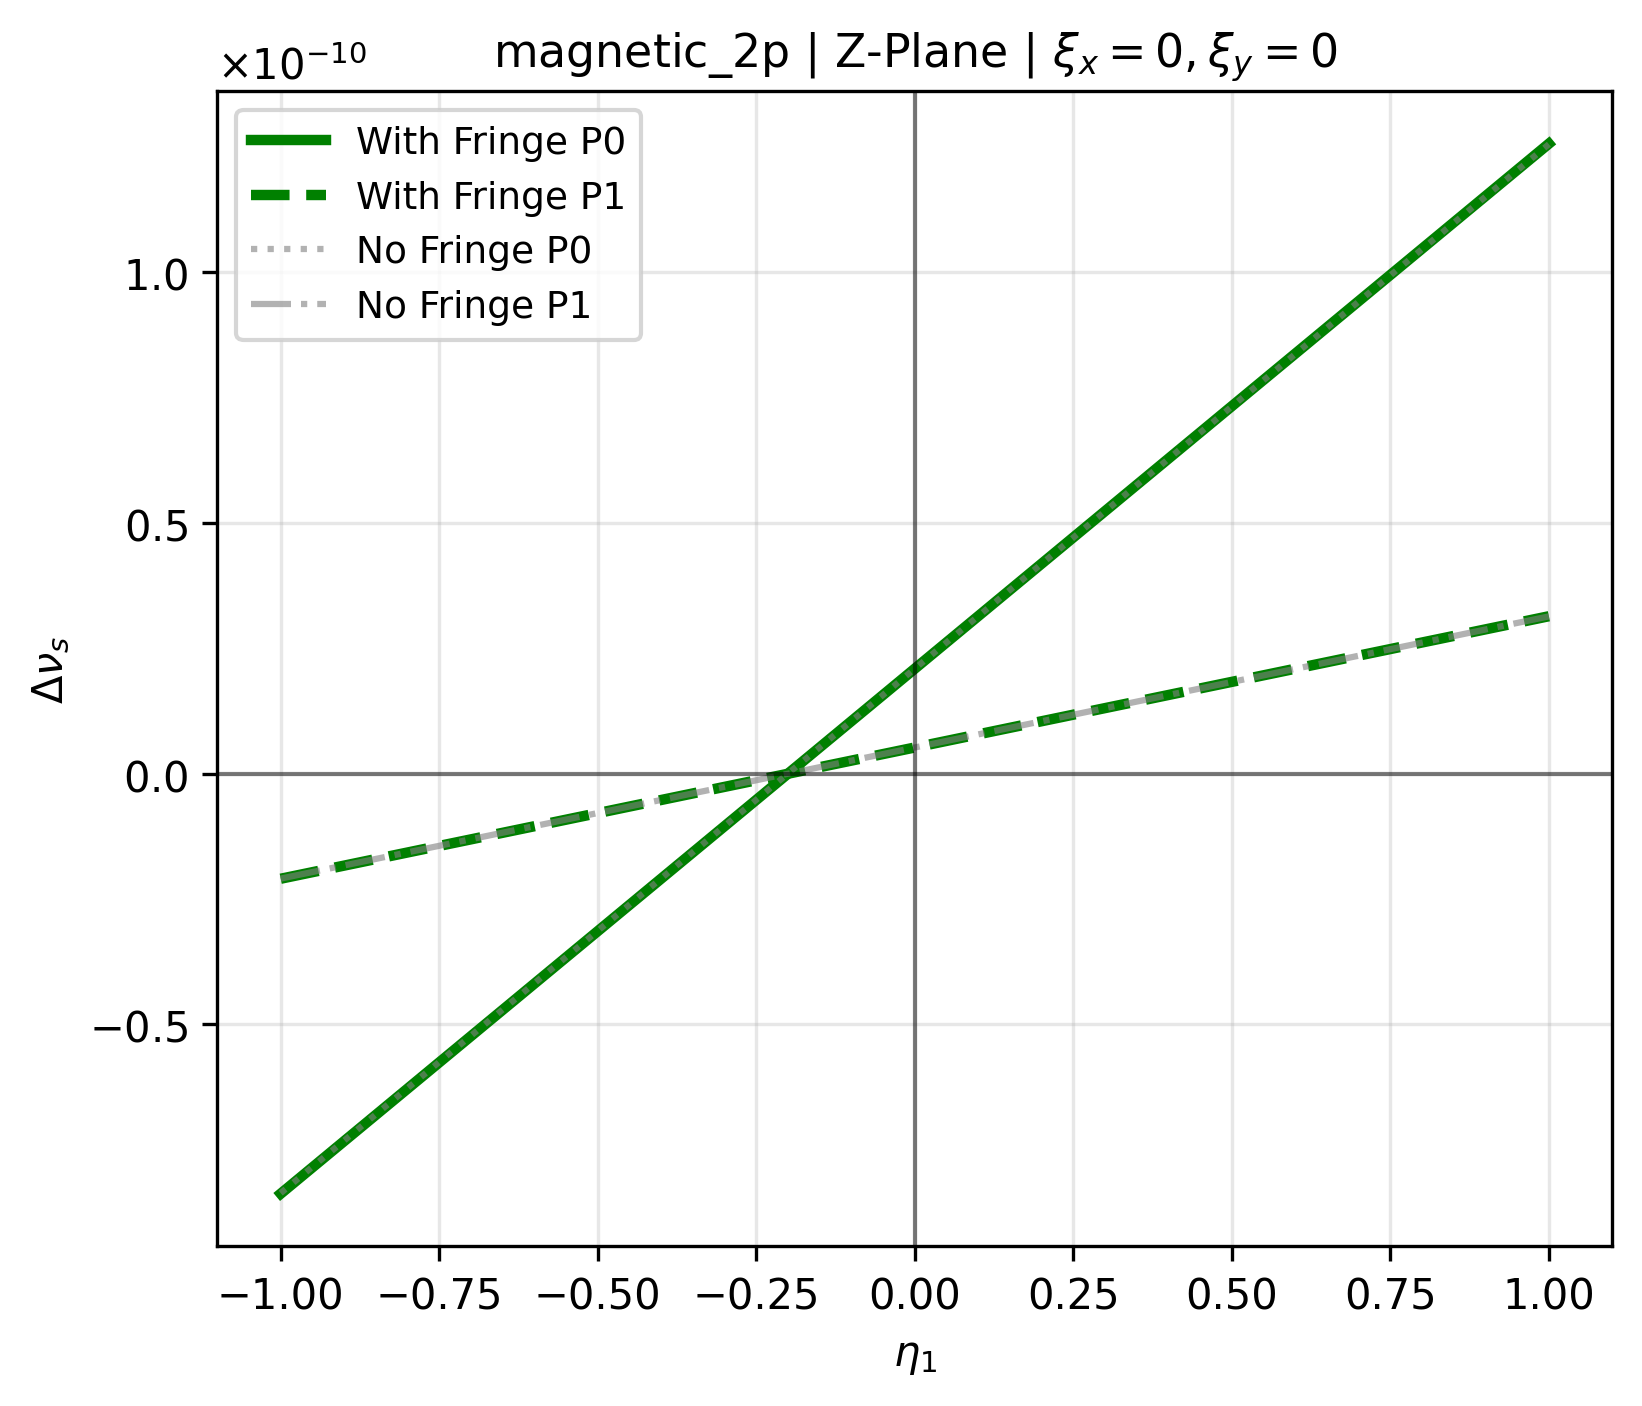
\includegraphics[width=\linewidth]{img/TUP3065_f2}
	\end{minipage}
	\caption{Magnet-only ring: \(\Delta\nu_s\) vs \(\xi_x\) (left) at \(\xi_y=0,\,\eta_1=0\) and vs \(\eta_1\) (right) at \(\xi_x=0,\,\xi_y=0\).}
	\label{fig:m2p_xz}
\end{figure}

\subsection{Electrostatic ring}
\par The electrostatic benchmark replaces magnetic bending/focusing with electrostatic elements; Twiss functions are in Fig.~\ref{fig:twiss_es}. The transfer slopes and intercepts move strongly relative to the magnet-only case~\cite{shankar23}.
\begin{figure}[!tbh]
	\centering
	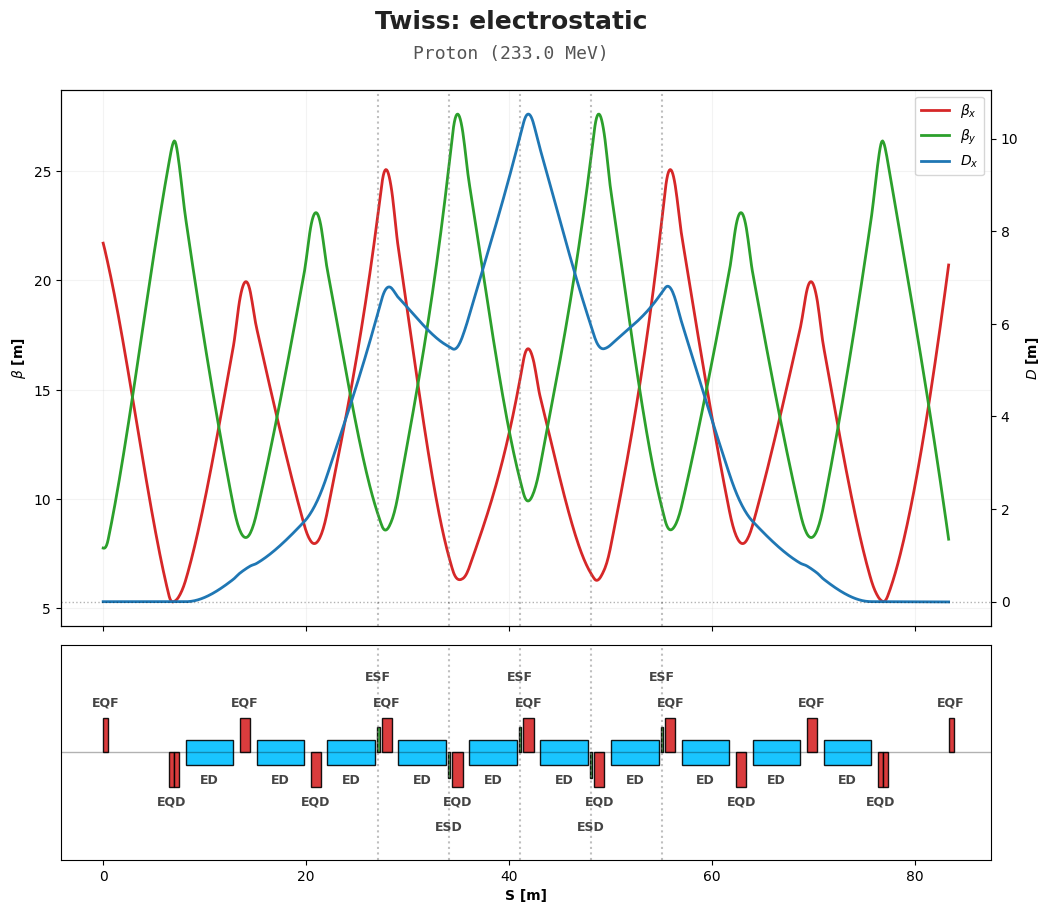
\includegraphics[width=\columnwidth]{img/TUP3065_f8}
	\caption{Electrostatic ring: Twiss functions.}
	\label{fig:twiss_es}
\end{figure}
\begin{figure}[!tbh]
	\centering
	\begin{minipage}[t]{0.49\columnwidth}
		\centering
		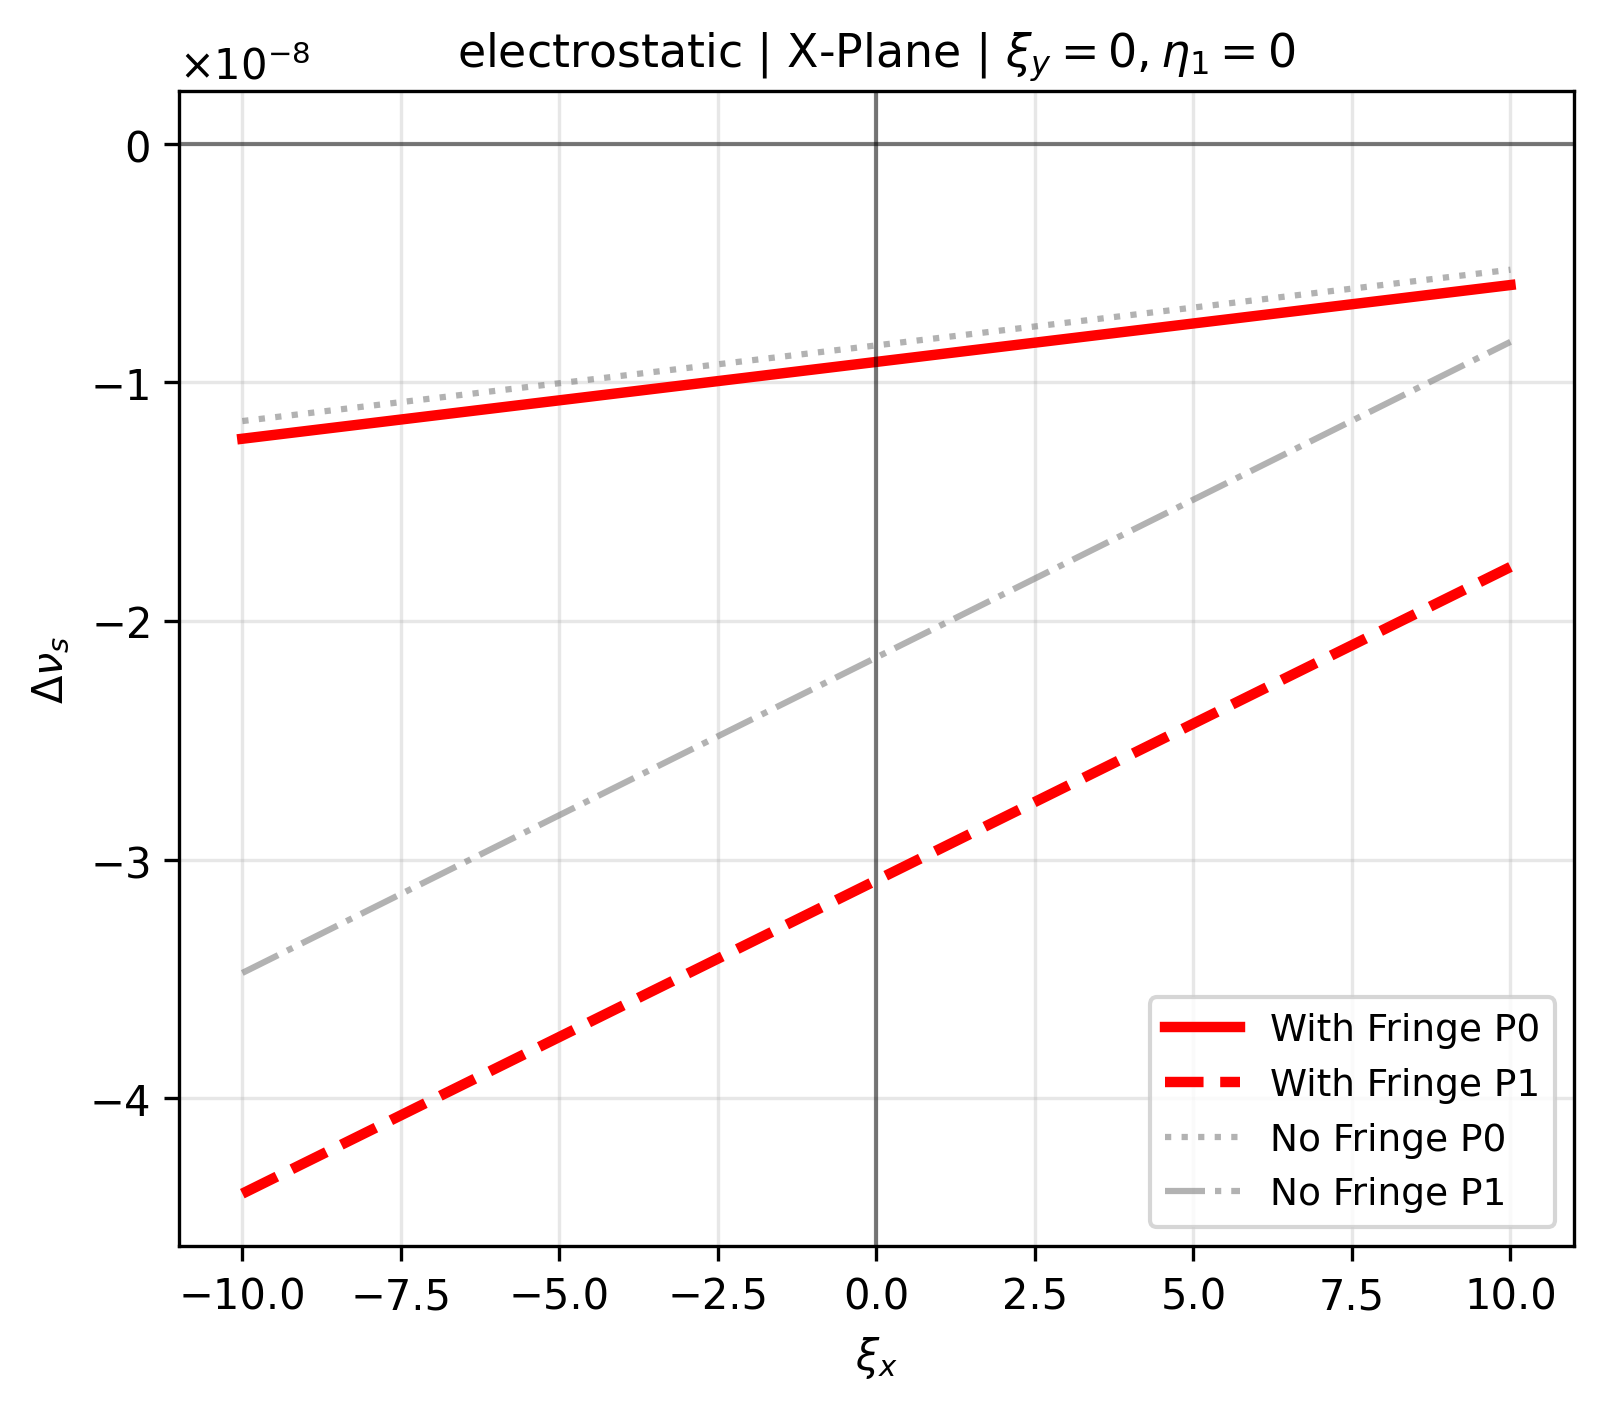
\includegraphics[width=\linewidth]{img/TUP3065_f3}
	\end{minipage}\hfill
	\begin{minipage}[t]{0.49\columnwidth}
		\centering
		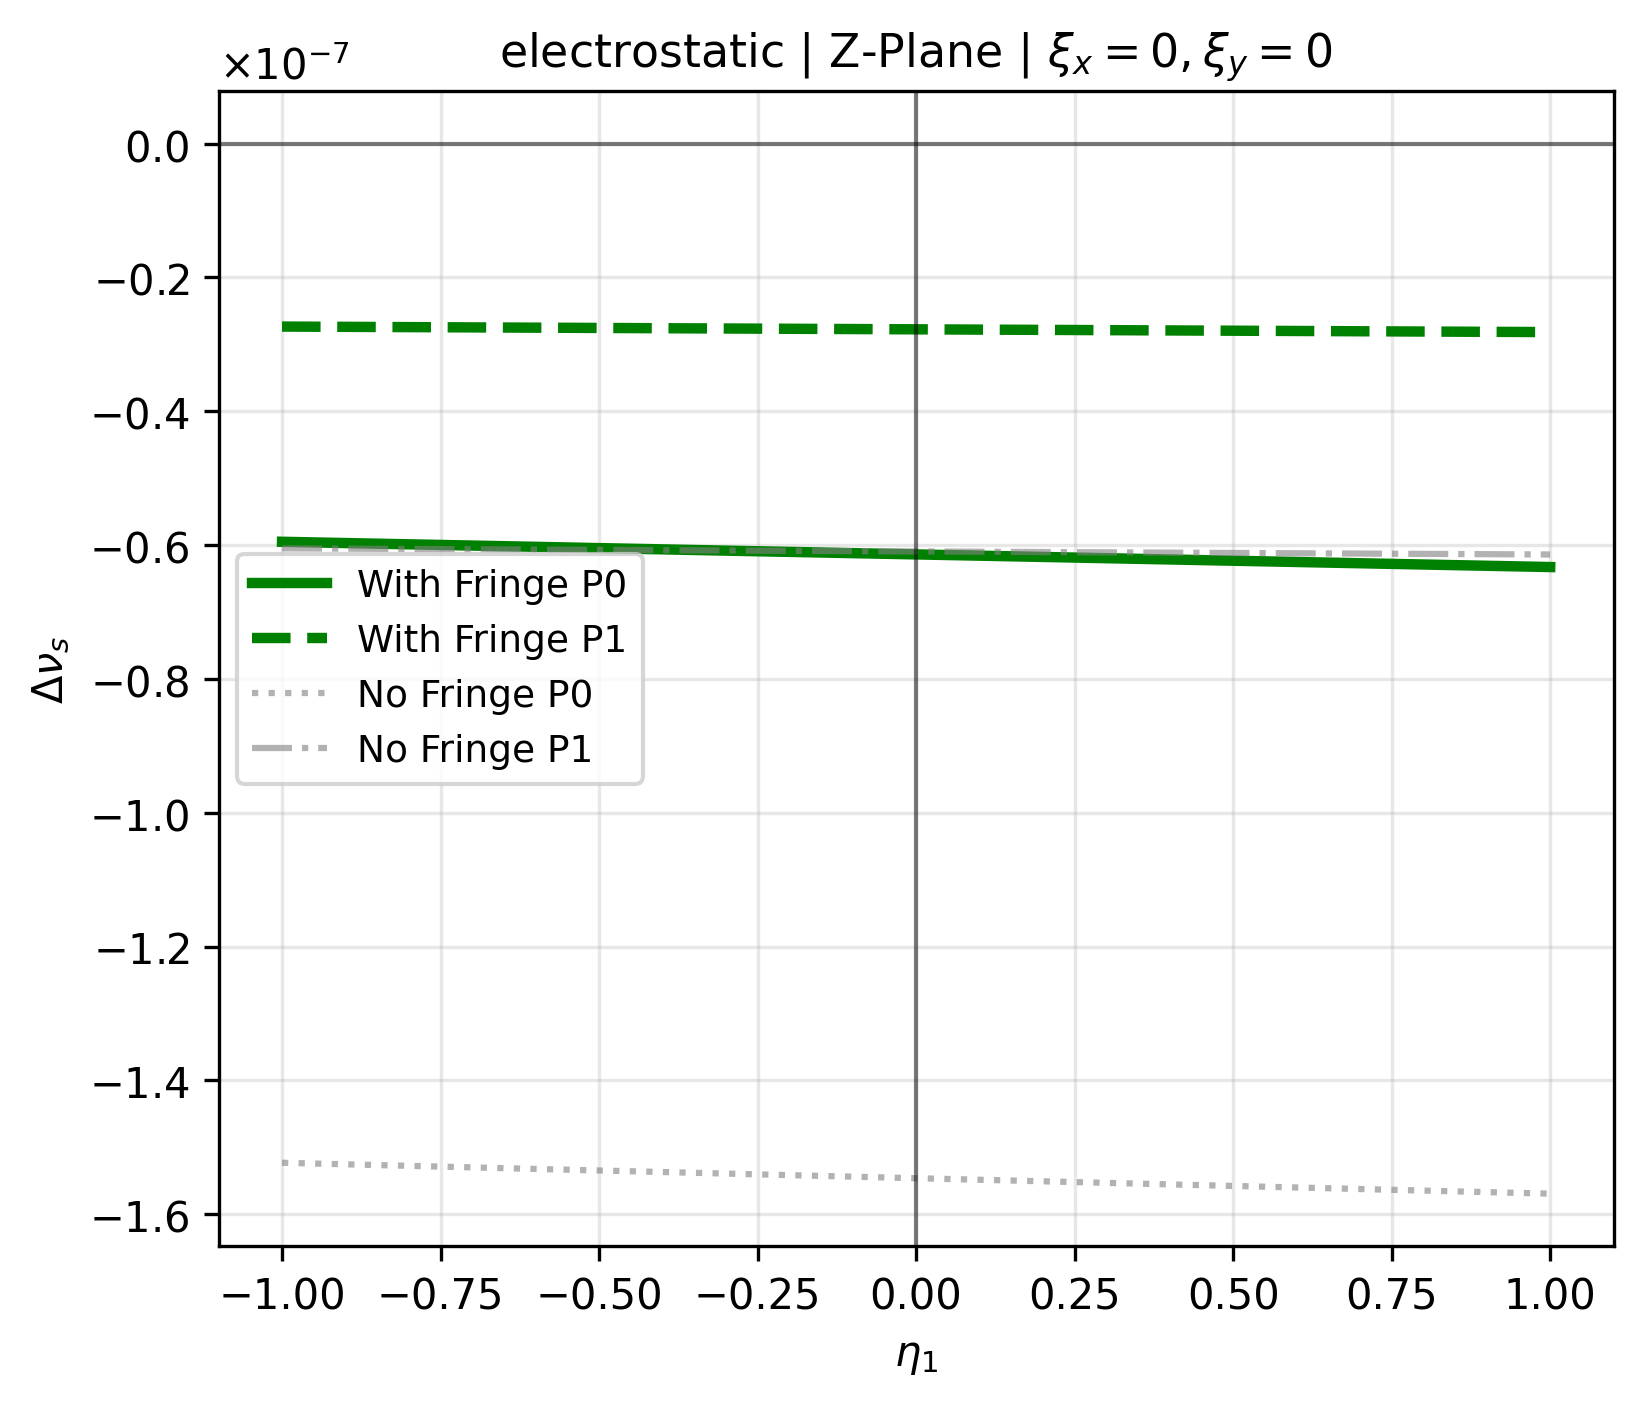
\includegraphics[width=\linewidth]{img/TUP3065_f4}
	\end{minipage}
	\caption{Electrostatic ring: \(\Delta\nu_s\) vs \(\xi_x\) (left) at \(\xi_y=0,\,\eta_1=0\) and vs \(\eta_1\) (right) at \(\xi_x=0,\,\xi_y=0\).}
	\label{fig:es_xz}
\end{figure}

\subsection{Combined-function QFS ring}
\par The combined-function benchmark is a quasi-frozen-spin (QFS) layout with electric and magnetic bends and straight Wien filters on the reference orbit; Twiss functions are in Fig.~\ref{fig:twiss_n8}. The same sextupole scan and decoupled chromatic targets apply as for the other two rings.
\begin{figure}[!tbh]
	\centering
	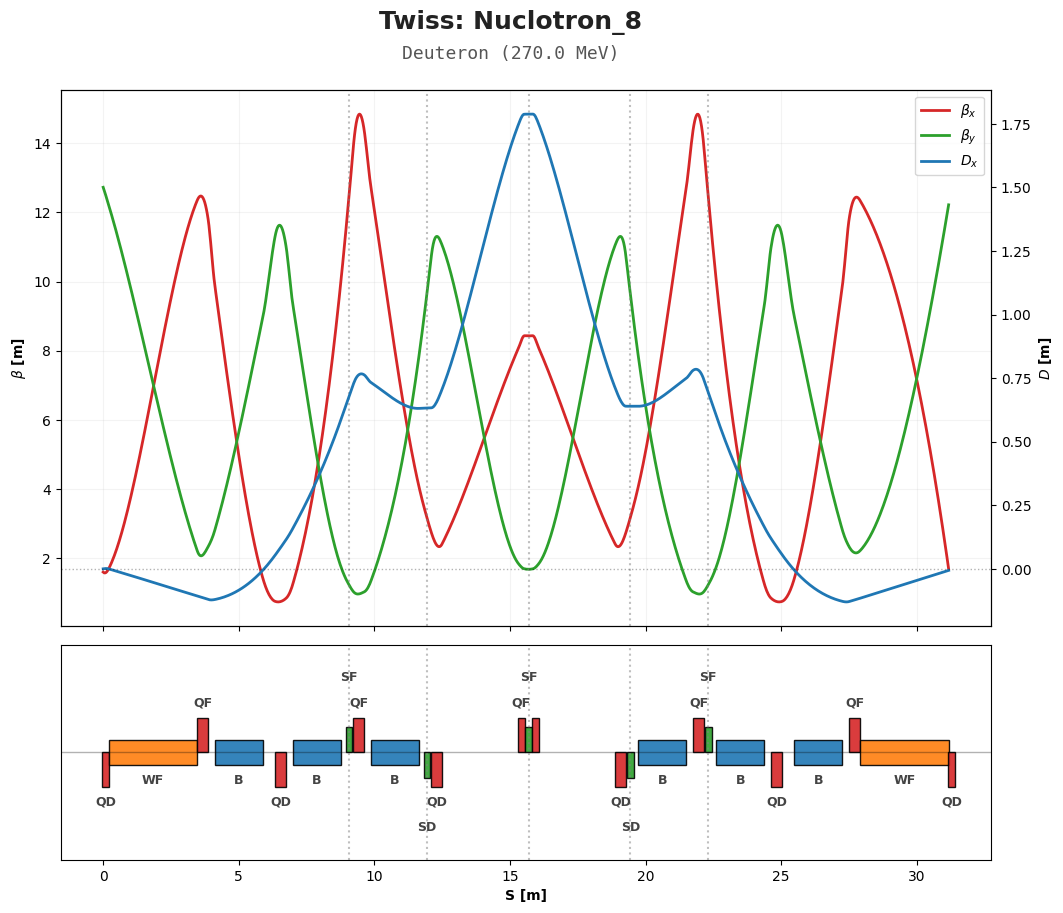
\includegraphics[width=\columnwidth]{img/TUP3065_f9}
	\caption{Combined-function QFS ring: Twiss functions.}
	\label{fig:twiss_n8}
\end{figure}
\begin{figure}[!tbh]
	\centering
	\begin{minipage}[t]{0.49\columnwidth}
		\centering
		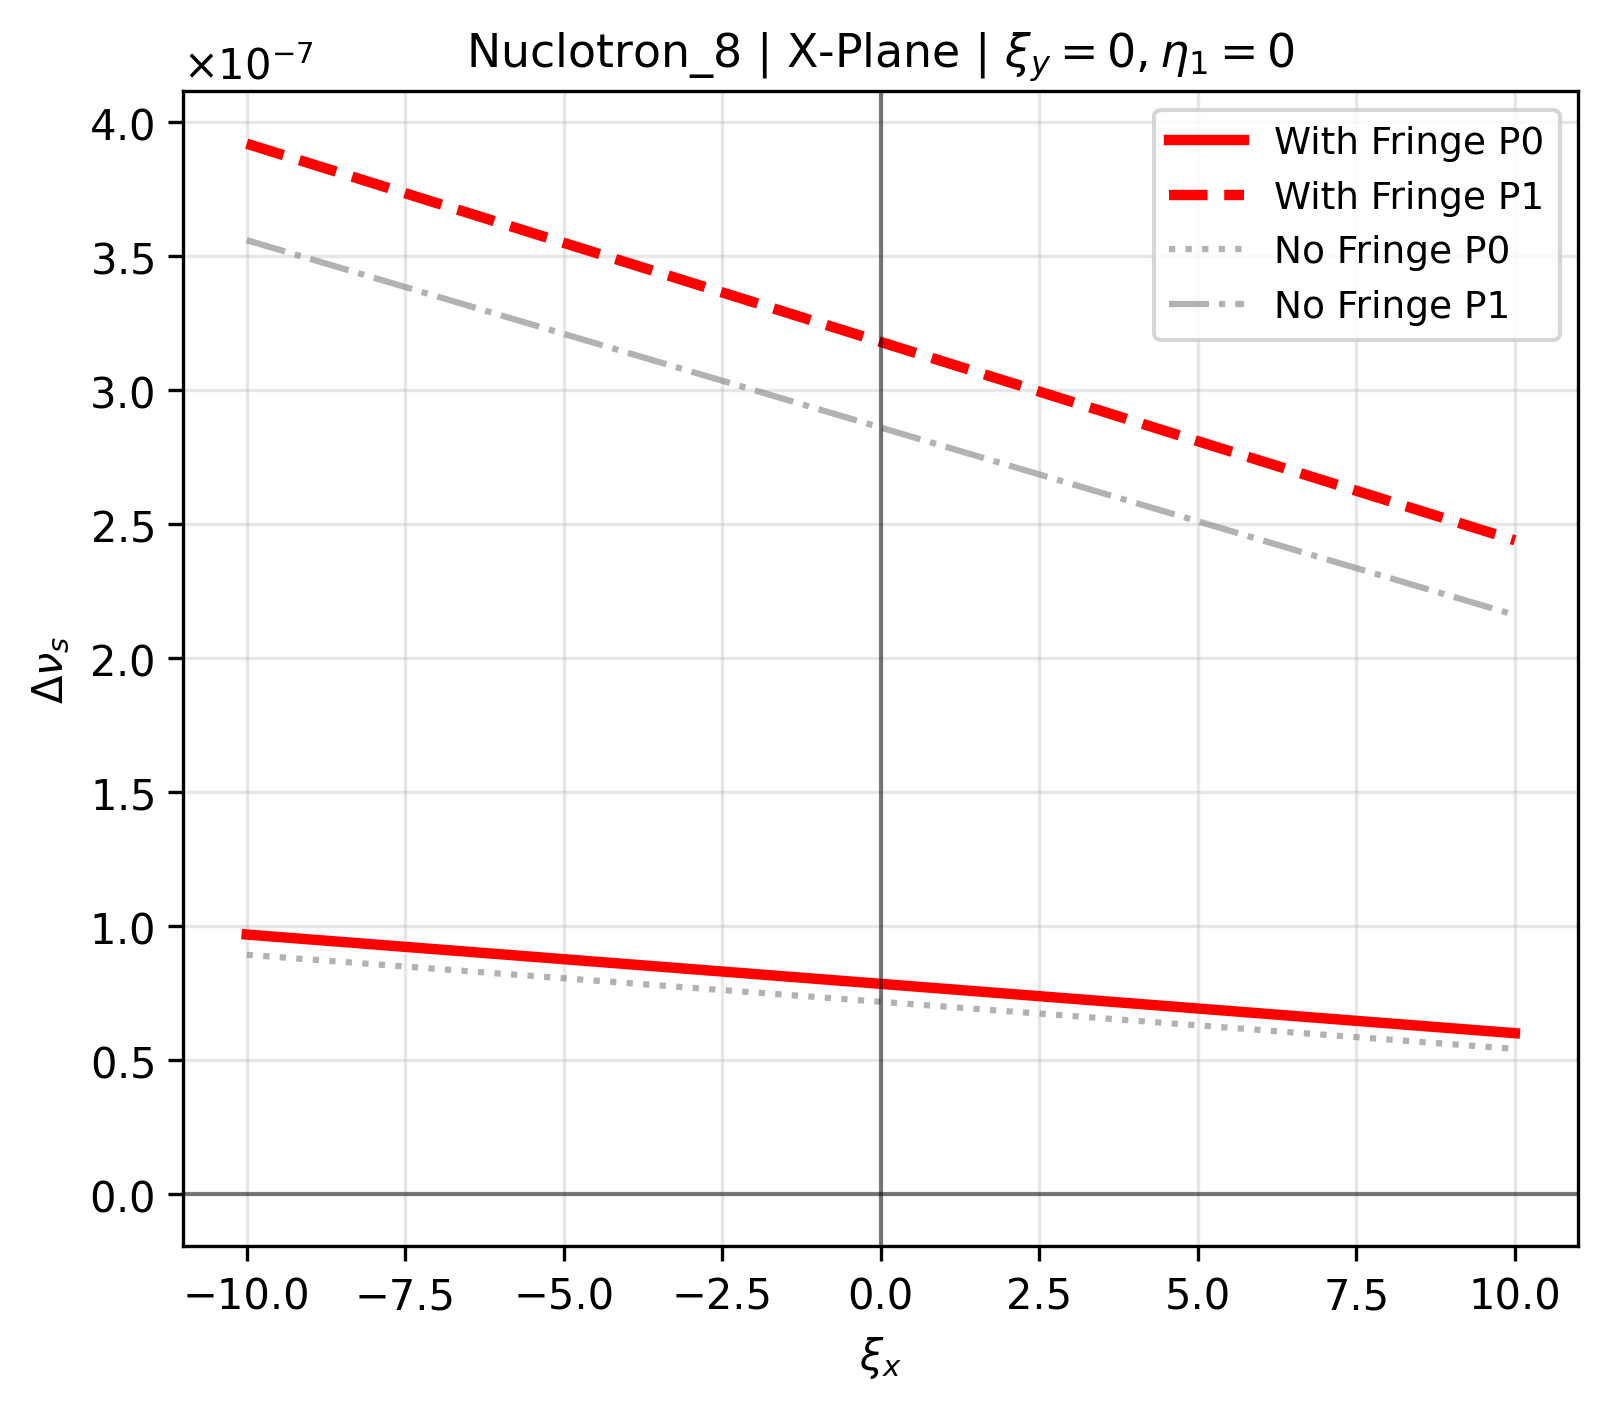
\includegraphics[width=\linewidth]{img/TUP3065_f5}
	\end{minipage}\hfill
	\begin{minipage}[t]{0.49\columnwidth}
		\centering
		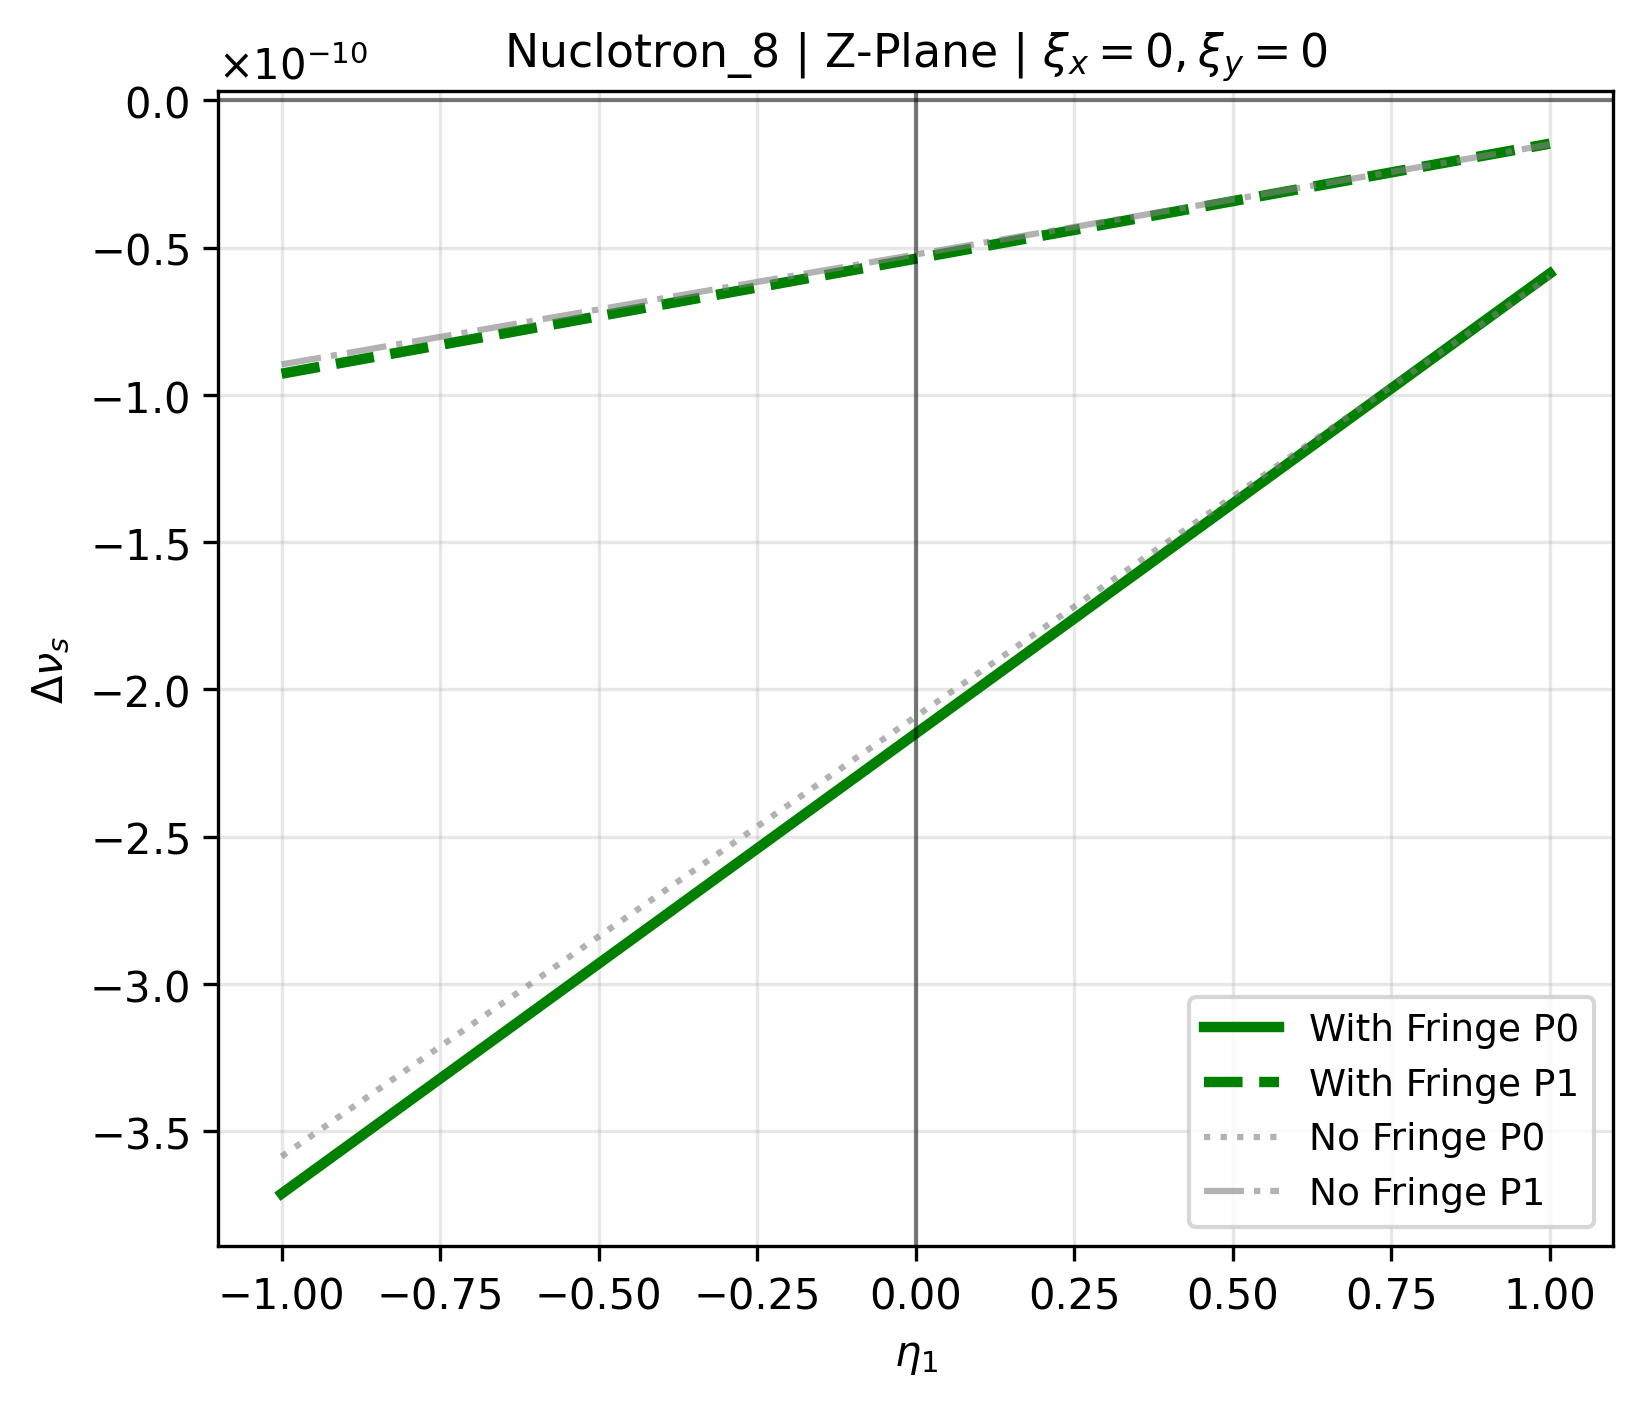
\includegraphics[width=\linewidth]{img/TUP3065_f6}
	\end{minipage}
	\caption{Combined-function QFS ring: \(\Delta\nu_s\) vs \(\xi_x\) (left) at \(\xi_y=0,\,\eta_1=0\) and vs \(\eta_1\) (right) at \(\xi_x=0,\,\xi_y=0\).}
	\label{fig:n8_xz}
\end{figure}

\section{Results and discussion}
\par The three lattices differ only in the baseline magneto-optics; the same three sextupole families and the same current grid are scanned in every case, so the spread of curves in Figs.~\ref{fig:m2p_xz}--\ref{fig:n8_xz} reflects how the underlying ring---magnetic, electrostatic, or QFS with Wien filters---changes the coupling between chromatic corrections and the spin-tune deviation \(\Delta\nu_s\). The dominant message is qualitative: electrostatic and combined-function arcs tilt and offset the transfer lines much more than the magnet-only reference, in agreement with other EDM-ring studies~\cite{shankar23}.

\par The two alternative initial conditions probe whether a single linearisation in \(\vec I\), trained at the smaller offsets, still tracks the spin response when the transverse starting amplitude is doubled and the fractional \(\Delta K/K\) excursion is halved. When the two post-hoc straight-line fits versus a given chromatic coordinate remain close at the working point, the Jacobian model is usable across that amplitude window; a visible split indicates stronger non-linearity or coupling outside the three-family corrector space. In operation one would pick chromatic targets along the decoupled scans of Eq.~(\ref{eq:constraints}), read off the implied sextupole currents from the fitted chromatic response, and inspect the predicted \(\Delta\nu_s\) before applying currents to hardware. Scripts and lattice files are in Ref.~\cite{sctrepo}.

\section{Conclusion}
\par The mapping approach used here is built directly from dense scans of the three sextupole families: for each current triplet, COSY records chromaticities, the longitudinal chromatic integral, and spin-tune deviations for several off-reference probes. Ordinary least squares turns those tables into straight-line laws linking currents to chromatics and to \(\Delta\nu_s\); combining the two fits yields the spin response as a function of chromatic targets without hand-tuning the magnets on a one-by-one basis. Everything stays tied to real family currents on the power supplies.

\par Spin-tune offsets are quoted relative to the stored reference particle. Each panel overlays the linear predictions obtained for the two initial-condition sets; agreement between them at the target chromaticity indicates that the mapped correction is stable across that amplitude window. Switching the ring from an all-magnetic baseline to electrostatic or QFS optics moves the trends dramatically.

\par Future work will look at how the periodicity of the arc layout affects the same \(\Delta\nu_s\) signatures when the three-family corrector layout is carried over to longer or more symmetric structures.

\section{Acknowledgements}

\par Support of this study by the Russian Science Foundation grant 25-72-30005 is acknowledged.

\ifboolexpr{bool{jacowbiblatex}}
	{\printbibliography}
	{
	\begin{thebibliography}{99}
	
	\bibitem{melnikov22}
	A.~A. Melnikov, A.~E. Aksentyev, Y.~Senichev, and E.~Syresin,
	``Investigation of Polarized Proton Spin Coherence Time at Storage Rings,''
	in \textit{Proc. 13th Int. Particle Accel. Conf. (IPAC'22)}, Bangkok, Thailand, Jun. 2022, paper WEPOPT005, pp.~1832--1834.
	\url{https://doi.org/10.18429/JACoW-IPAC2022-WEPOPT005}.
	
	\bibitem{senichev25}
	Y.~V. Senichev, S.~D. Kolokolchikov, A.~E. Aksentyev, \emph{et al.},
	``Modernization of the Magneto-Optical Structure of the Nuclotron to Study the Possibility of Measuring the Electric Dipole Moment of Light Nuclei with Preservation of Functions of the Booster of Polarized Beams for the NICA Collider,''
	Phys. At. Nucl. \textbf{88}, 2025--2034 (2025).
	\url{https://doi.org/10.1134/S1063778825100370}.
	
	\bibitem{shankar23}
	R.~Shankar, P.~Lenisa, and A.~Lehrach,
	``Optimization of spin-coherence time for electric dipole moment measurements in a storage ring,''
	PoS \textbf{PSTP2022} (2023) 024.
	\url{https://doi.org/10.22323/1.433.0024}.
	
	\bibitem{guidoboni18}
	G.~Guidoboni \emph{et al.} (JEDI Collaboration),
	``Connection between zero chromaticity and long in-plane polarization lifetime in a magnetic storage ring,''
	Phys. Rev. Accel. Beams \textbf{21}, 024201 (2018).
	\url{https://doi.org/10.1103/PhysRevAccelBeams.21.024201}.
	
	\bibitem{cosy}
	K.~Makino and M.~Berz,
	``COSY INFINITY version 9,''
	Nucl. Instrum. Methods Phys. Res. A \textbf{558} (2006) 346--350;
	COSY INFINITY portal, Michigan State University.
	\url{https://www.bmtdynamics.org/cosy/}.
	
	\bibitem{sctrepo}
	``SCT---Optimization on Spin Coherence Time,'' public code repository (COSY scripts, notebooks, data reduction, and lattice files),
	\url{https://github.com/sergeybell/SCT}.
	
	\end{thebibliography}
}

\end{document}